%==============================================================================
%  RehabSense — Product Requirements Document  v1.5
%  CSE/EE 475 Embedded Systems Capstone + EE 542, Autumn 2026, Team 1
%  Compile with pdfLaTeX on Overleaf. Self-contained: no external image files.
%
%  EDIT THESE LINES AND YOU ARE DONE:
%==============================================================================
\newcommand{\ProjectTitle}{RehabSense}
\newcommand{\ProjectSub}{A wearable sEMG + IMU sleeve for home-based stroke rehabilitation}
\newcommand{\CourseLine}{CSE/EE 475 — Embedded Systems Capstone \,/\, EE 542 \quad\textbullet\quad
                         Team 1 \quad\textbullet\quad Autumn 2026}
\newcommand{\TeamLine}{Qian (Andy) Cai \quad\textbullet\quad Eyerusalem Earl \quad\textbullet\quad
                       Rusha Maiti \quad\textbullet\quad Aidan Goodman}
\newcommand{\InstructorLine}{Instructor: Prof.\ Shwetak N.\ Patel \quad\textbullet\quad
                             TAs: Alex Ching, Guilin Hu}
%==============================================================================

\documentclass[11pt]{article}

% ---------- page ----------
\usepackage[letterpaper,margin=1in,headheight=14pt]{geometry}
\usepackage[T1]{fontenc}
\usepackage[utf8]{inputenc}
\IfFileExists{lmodern.sty}{\usepackage{lmodern}}{}
\IfFileExists{XCharter.sty}{\usepackage[scaled=1.0]{XCharter}}{}
\IfFileExists{FiraSans.sty}{\usepackage[sfdefault,scaled=0.92]{FiraSans}}{}
\IfFileExists{lmodern.sty}{\usepackage{microtype}}{\usepackage[expansion=false]{microtype}}

\usepackage{amsmath}
\usepackage{graphicx}
\usepackage{float}
\usepackage{array}
\usepackage{booktabs}
\usepackage{tabularx}
\usepackage{enumitem}
\usepackage[table]{xcolor}
\usepackage{titlesec}
\usepackage{fancyhdr}
\usepackage[most]{tcolorbox}
\usepackage{caption}
\usepackage{tikz}
\usetikzlibrary{arrows.meta,positioning,decorations.pathmorphing,shapes.geometric,calc,fit,backgrounds}
\usepackage[hidelinks]{hyperref}

% ---------- palette ----------
\definecolor{ink}{HTML}{1C1C1C}
\definecolor{marker}{HTML}{E4572E}
\definecolor{annot}{HTML}{2E5EAA}
\definecolor{paper}{HTML}{FAF7F2}
\definecolor{rule}{HTML}{D8D2C8}
\definecolor{soft}{HTML}{6E6A64}
\definecolor{limb}{HTML}{DAD4CA}
\definecolor{good}{HTML}{2F7A52}

\color{ink}

% ---------- headings ----------
\titleformat{\section}{\normalfont\large\bfseries\color{ink}}{\color{marker}\thesection}{0.8em}{}
\titlespacing*{\section}{0pt}{1.6em}{0.6em}
\titleformat{\subsection}{\normalfont\normalsize\bfseries\color{ink}}{\color{soft}\thesubsection}{0.7em}{}
\titlespacing*{\subsection}{0pt}{1.2em}{0.4em}
\titleformat{\subsubsection}[runin]{\normalfont\bfseries\color{ink}}{}{0pt}{}[.\hspace{0.4em}]

\setlist[itemize]{leftmargin=1.2em,itemsep=2pt,topsep=4pt}
\setlist[enumerate]{leftmargin=1.4em,itemsep=2pt,topsep=4pt}

\pagestyle{fancy}\fancyhf{}
\renewcommand{\headrulewidth}{0.4pt}
\fancyhead[L]{\small\color{soft}\ProjectTitle\ — PRD v1.5}
\fancyhead[R]{\small\color{soft}\thepage}

\captionsetup{font=small,labelfont={bf,color=soft},textfont=it,width=0.9\linewidth}

% ---------- callout boxes ----------
\newtcolorbox{callout}[1][]{
  enhanced, breakable, colback=paper, colframe=rule, boxrule=0.6pt,
  arc=2pt, left=10pt, right=10pt, top=8pt, bottom=8pt, #1}

\newtcolorbox{phasebox}[1]{
  enhanced, breakable, colback=marker!6, colframe=marker, boxrule=1pt, arc=2pt,
  left=10pt,right=10pt,top=8pt,bottom=8pt,
  fonttitle=\bfseries\sffamily, title={#1}, coltitle=white, colbacktitle=marker}

\newtcolorbox{plainbox}{
  enhanced, breakable, colback=white, colframe=ink, boxrule=1pt, arc=2pt,
  left=10pt,right=10pt,top=8pt,bottom=8pt}

\newcommand{\tested}{{\sffamily\scriptsize\color{good}\textbf{[21 Oct test]}}\ }

% ---------- tikz styles ----------
\tikzset{
  fat/.style   ={line width=2.4pt, color=marker, line cap=round, line join=round,
                 decorate, decoration={random steps, segment length=7mm, amplitude=0.22pt}},
  lead/.style  ={line width=0.7pt, color=annot, -{Stealth[length=4pt]}},
  note/.style  ={font=\sffamily\scriptsize, color=annot, align=left, inner sep=1.5pt},
  place/.style ={draw=ink, line width=1pt, rounded corners=2pt, fill=white,
                 align=left, inner sep=6pt, font=\sffamily\scriptsize, minimum width=30mm},
  flow/.style  ={-{Stealth[length=5pt]}, line width=0.9pt, color=ink},
  st/.style    ={draw=marker, line width=1.3pt, rounded corners=3pt, fill=marker!6,
                 align=center, inner sep=4pt, font=\sffamily\scriptsize, minimum width=22mm},
  blk/.style   ={draw=ink, line width=0.9pt, rounded corners=2pt, fill=white,
                 align=center, inner sep=4pt, font=\sffamily\scriptsize, minimum height=9mm},
}

\newcommand{\afford}[1]{\underline{\smash{#1}}}

\begin{document}

%==============================================================================
\begin{center}
{\LARGE\bfseries \ProjectTitle}\\[2pt]
{\large\color{soft} \ProjectSub}\\[10pt]
{\small \CourseLine}\\[2pt]
{\small \TeamLine}\\[2pt]
{\small\color{soft} \InstructorLine}\\[2pt]
{\small\color{soft} PRD v1.5 \quad\textbullet\quad October 22, 2026 \quad\textbullet\quad
\href{https://sites.google.com/uw.edu/ee542group1-rehabsense/timeline}{project site}}
\end{center}
\vspace{4pt}
{\color{rule}\hrule height 1pt}
\vspace{10pt}

%==============================================================================
\section{Summary}

RehabSense is a low-cost wearable sleeve for home-based stroke rehabilitation
that measures muscle activity and limb motion at the same time, grades each
exercise repetition on the device, and tells the patient the result through a
vibration on their own arm. A surface-EMG channel on the biceps and two
inertial sensors on the upper arm and forearm let the system distinguish a
repetition genuinely performed by the target muscle from one completed by
shoulder elevation, trunk lean, or momentum --- a distinction that motion-only
rehabilitation devices cannot make and that no one is present to make at home.
Each repetition receives a 0--100 score built from range of motion, tempo, and
smoothness, together with a fatigue indicator derived from the EMG frequency
spectrum. A second channel on the triceps arrives with the custom PCB and adds
co-contraction as a fourth scored component. Results stream over Bluetooth Low Energy to a host
application for the patient and, eventually, their therapist. The quarter
delivers a working wearable prototype on a custom PCB, demonstrated live.

\begin{callout}
\textbf{Document status.} This revision incorporates measurements from a working
prototype exercised on a volunteer on 21 October (ESP32 DevKit, 2 $\times$
BMI270, MyoWare 2.0, DRV2605L driving an ERM actuator). Findings from that
session are tagged \tested throughout, distinguishing measured values from
assumed ones.

\medskip
\textbf{What changed in v1.5.} Four decisions taken on 22 October, after the
firmware had been brought into line with v1.4:

\begin{itemize}
\item \textbf{One EMG channel for the prototype.} A single MyoWare 2.0 on the
biceps --- two electrodes on the muscle belly plus one reference at the elbow,
three in all. The triceps channel, and with it the co-contraction score,
arrives with the custom PCB.
\item \textbf{The ERM is the production actuator.} The move to an LRA,
proposed in v1.4, is reversed; every LRA reference is removed.
\item \textbf{A soft click at 80\% of the target angle} is added --- an open
question in v1.4, now settled yes.
\item \textbf{A fatigue warning advises and does not end the set} --- the
other open question, settled the same way.
\end{itemize}

\medskip
\textbf{Implementation status.} Firmware implementing this document is in the
repository at \texttt{cse475/firmware}, with the design recorded in
\emph{Firmware Design v2.0}. Everything specified here is built: the
activation-gated repetition cycle, grading, the seven-pattern haptic
vocabulary with priority and preemption, the five-step calibration protocol,
the full BLE command set including runtime configuration, and backfill after a
dropout.

\medskip
Five test suites run on a laptop with no hardware, no radio and no ESP-IDF,
and all five pass. The repetition suite compiles the real
\texttt{rep\_cycle.c}, \texttt{grading.c} and \texttt{activation.c} and
drives sixteen scenarios through them, including a passively swung arm that
counts nothing. What remains outstanding needs a bench, volunteer data, or a
team decision; none of it is firmware work. The custom PCB is in design.
\end{callout}

%==============================================================================
\section{Problem statement}

Stroke is among the most common causes of long-lasting upper-limb impairment.
The CDC reports that more than 795{,}000 people in the United States have a
stroke each year, that stroke is a leading cause of serious long-term
disability, and that it reduces mobility in more than half of survivors aged 65
and above~\cite{cdc}. Recovery of arm function depends on sustained,
high-repetition practice, the majority of which is prescribed as a home exercise
programme and performed without supervision between clinical visits.

Unsupervised practice introduces two failure modes that neither the patient nor
the therapist can currently observe.

\begin{itemize}
\item \textbf{Compensatory movement.} When the target muscle cannot generate
sufficient force, the movement is completed by recruiting other structures ---
elevating the shoulder, leaning the trunk, or using momentum. The joint
trajectory still appears complete, but the intended muscle performs little of
the work. Because the substitution is repeated across many sessions, it is
reinforced as a motor pattern and becomes progressively harder to correct.
\item \textbf{Unmonitored fatigue.} Repetition quality degrades as the muscle
fatigues, and fatigued practice contributes disproportionately to compensatory
patterns. No objective indicator currently tells a patient when to rest or a
therapist how much of a prescribed session was performed under fatigue.
\end{itemize}

Both failure modes are invisible in the dominant documentation method --- a
self-reported repetition count on paper --- so the clinician returns to a session
with no information about how the preceding weeks of practice were actually
performed.

\begin{table}[H]
\centering\small
\begin{tabularx}{\linewidth}{@{}>{\raggedright\arraybackslash}p{0.27\linewidth} X@{}}
\toprule
\textbf{Existing approach} & \textbf{Limitation for unsupervised home practice} \\
\midrule
Paper home-exercise programmes & No feedback mechanism; adherence and movement quality are both unrecorded. \\
Camera- and IMU-based rehabilitation games & Measure kinematics only. Cannot determine whether the target muscle was recruited, cannot observe fatigue, and score compensated movements as successful. \\
Clinic-based rehabilitation robots and exoskeletons & Accurate and well validated, but expensive, non-wearable, and dependent on travel to a facility. \\
Therapist-supervised EMG biofeedback units & Observe muscle activity accurately, but are stationary, typically single-channel, and are not designed to score exercise repetitions. \\
\bottomrule
\end{tabularx}
\end{table}

\begin{callout}
\textbf{Gap addressed by this project.} Kinematic measurement alone can be
satisfied by a compensated movement; electromyography alone cannot localise
where a movement originated. No low-cost wearable system currently measures both
simultaneously and returns feedback to the patient within the session in which
the error occurs.
\end{callout}

\noindent
\textbf{Target applications.} Home rehabilitation with real-time movement-quality
feedback; tele-rehabilitation, in which objective session data is reviewed
remotely; a clinic-to-home bridge that records progress between appointments;
and a low-cost research platform for rehabilitation studies.

%==============================================================================
\section{Deliverables and critical features}

\subsection{What will be demonstrated on 10 December}

\begin{enumerate}
\item A wearable sleeve carrying one EMG channel, two IMUs, and a haptic
actuator, driven by a custom PCB in a 3D-printed pod with its own battery, power
switch, user button, and status LED.
\item A live session: don the sleeve, pass the contact check, run calibration,
and perform a set of repetitions with the counter advancing and a haptic
response on each one.
\item Deliberate compensation --- shoulder elevation --- detected live, flagged
with a distinct haptic pattern, reflected in a lowered score, and named on the
host display.
\item A passively swung arm rejected: no repetition starts, because the biceps
never activates.
\item A fatiguing set, with the median-frequency trend falling and the rest cue
firing.
\item Exercise parameters --- hold duration, repetition target, target angle ---
changed live from the host application.
\item The host application showing live traces, per-repetition scores, and a
session summary.
\end{enumerate}

\subsection{Critical features}

\begin{table}[H]
\centering\small
\begin{tabularx}{\linewidth}{@{}p{46mm} p{20mm} X@{}}
\toprule
\textbf{Feature} & \textbf{Priority} & \textbf{Notes} \\
\midrule
Single-channel sEMG acquisition & Must & Biceps; raw, band-limited. The triceps channel arrives with the custom PCB \\
Dual-IMU elbow angle & Must & Relative orientation, $5$--$10^{\circ}$ accuracy \\
On-device repetition detection & Must & Deterministic; gated on biceps activation \\
On-device grading, 0--100 & Must & Three equal-weight components; a fourth with the second channel \\
Compensation detection & Must & Shoulder elevation, trunk lean, momentum \\
Haptic feedback, three outcomes & Must & Clean, flagged, set complete; distinct by rhythm \\
Movement waypoint cue & Should & Soft click at 80\% of the target angle \\
Fault and rest cues & Must / Should & Fault is a must (contact loss, sensor error, low battery); the fatigue rest cue is a should \\
Non-overlapping cue playback & Must & Single-slot priority queue; a fault preempts a playing cue \\
Driver configuration self-test & Must & Register read-back before every session \\
Host pattern test & Should & Named pattern fired on demand for bench and volunteer testing \\
BLE streaming and control & Must & Live features, events, switchable raw stream \\
Host application & Must & Python for the prototype; Flutter thereafter \\
Calibration under 30\,s & Must & Six prompted steps, individually repeatable \\
Fatigue detection & Should & Median-frequency regression across the set; advises, does not end the set \\
Custom PCB & Should & Development board is the fallback \\
Battery operation, 2\,h & Should & LiPo with fuel gauge \\
Enclosure and sleeve integration & Should & 3D-printed pod \\
Therapist dashboard & Could & Backend topics exercised; UI is later work \\
\bottomrule
\end{tabularx}
\end{table}

%==============================================================================
\section{Scope and phasing}

\begin{phasebox}{Phase 1 — rapid prototype, due on the project website 29 October, noon}
A functional benchtop prototype built on the ESP32-S3 development board with a
MyoWare 2.0 sensor, demonstrating the complete signal path: one EMG channel and
two IMUs acquired on a shared timebase, elbow angle derived to within
$5$--$10^{\circ}$, repetitions detected and graded on-device, the correct haptic
pattern issued, and the full stream logged by the Python host over BLE.

\smallskip
Excluded from this phase: the custom PCB, the sleeve assembly, the enclosure,
the patient-facing game, and electrode-site optimisation.
\end{phasebox}

\begin{phasebox}{Phase 2 — wearable prototype, 29 October to 10 December}
Custom PCB designed, fabricated, and brought up; sensors integrated into a
compression sleeve; 3D-printed pod with power switch, button, and RGB status
LED; grading parameters tuned against recorded volunteer data; two hours of
battery operation; and a demonstration script that runs reliably twice in
succession.
\end{phasebox}

\noindent
The MyoWare 2.0 module is the sensing front end for Phase 1 only. The custom PCB
replaces it with an integrated two-channel analogue front end, taking the
electrode count from three to five: the triceps pair is added and the single
driven reference is shared. Firmware is written against an abstract acquisition
interface with both backends in place, so the change does not propagate above
the driver layer, and everything that needs a second channel is already written
and guarded on one constant rather than waiting to be added.

%==============================================================================
\section{System design}

\begin{callout}
\textbf{Design summary.} A wearable sleeve measures muscle activity and limb
motion concurrently, determines on-device whether each repetition was performed
correctly, and communicates the result to the patient through a vibration
pattern delivered at a predictable point in the movement.
\end{callout}

\subsection{Sensor and electrode placement}

\begin{figure}[H]
\centering
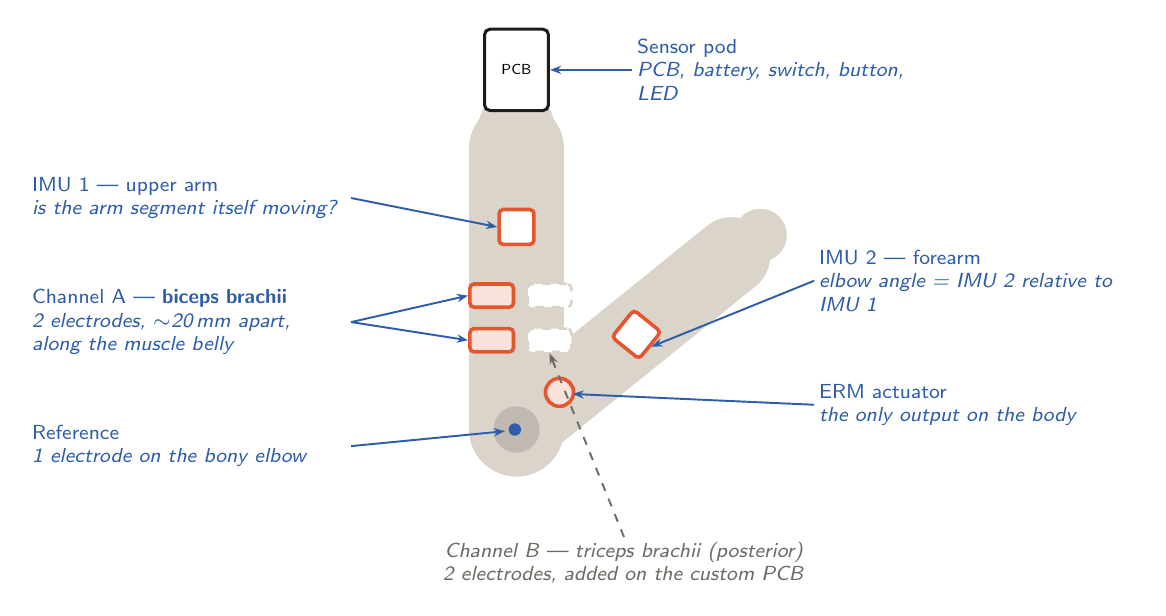
\begin{tikzpicture}[scale=1.05, every node/.style={transform shape}]

\draw[line width=34pt, limb, line cap=round] (0,0) -- (0,-3.4);
\draw[line width=28pt, limb, line cap=round] (0,-3.4) -- (2.6,-1.3);
\fill[limb] (0,0.25) circle (0.46);
\fill[limb!75!soft] (0,-3.4) circle (0.28);
\fill[limb] (2.95,-1.05) circle (0.32);

\node[draw=marker,line width=1.3pt,fill=white,rounded corners=1.5pt,
      minimum width=12pt,minimum height=12pt] (imuU) at (0,-0.95) {};
\node[draw=marker,line width=1.3pt,fill=white,rounded corners=1.5pt,
      minimum width=12pt,minimum height=12pt,rotate=-39] (imuF) at (1.45,-2.25) {};
\node[draw=marker,line width=1.3pt,fill=marker!18,rounded corners=1.5pt,
      minimum width=15pt,minimum height=8pt] (emgB) at (-0.30,-1.78) {};
\node[draw=marker,line width=1.3pt,fill=marker!18,rounded corners=1.5pt,
      minimum width=15pt,minimum height=8pt] (emgB2) at (-0.30,-2.32) {};
% Phase 2 only: the triceps pair the custom PCB adds.
\node[draw=rule,line width=0.9pt,dashed,fill=white,rounded corners=1.5pt,
      minimum width=15pt,minimum height=8pt] (emgT) at (0.40,-1.78) {};
\node[draw=rule,line width=0.9pt,dashed,fill=white,rounded corners=1.5pt,
      minimum width=15pt,minimum height=8pt] (emgT2) at (0.40,-2.32) {};
\draw[line width=1.3pt,marker,fill=marker!18] (0.52,-2.95) circle (0.17);
\node[draw=ink,line width=1.1pt,fill=white,rounded corners=2pt,
      minimum width=22pt,minimum height=28pt] (pod) at (0,0.95) {};
\node[font=\sffamily\tiny] at (0,0.95) {PCB};
\fill[annot] (-0.02,-3.40) circle (0.075);

\node[note,anchor=east,text width=38mm] (nU) at (-2.0,-0.60)
  {IMU 1 --- upper arm\\\textit{is the arm segment itself moving?}};
\draw[lead] (nU.east) -- (imuU.west);

\node[note,anchor=east,text width=38mm] (nB) at (-2.0,-2.10)
  {Channel A --- \textbf{biceps brachii}\\\textit{2 electrodes, $\sim$20\,mm apart,\\along the muscle belly}};
\draw[lead] (nB.east) -- (emgB.west);
\draw[lead] (nB.east) -- (emgB2.west);

\node[note,anchor=east,text width=38mm] (nRef) at (-2.0,-3.60)
  {Reference\\\textit{1 electrode on the bony elbow}};
\draw[lead] (nRef.east) -- (-0.14,-3.42);

\node[note,anchor=west,text width=38mm] (nP) at (1.4,0.95)
  {Sensor pod\\\textit{PCB, battery, switch, button, LED}};
\draw[lead] (nP.west) -- (pod.east);

\node[note,anchor=west,text width=38mm] (nF) at (3.6,-1.60)
  {IMU 2 --- forearm\\\textit{elbow angle = IMU 2 relative to IMU 1}};
\draw[lead] (nF.west) -- (imuF.east);

\node[note,anchor=west,text width=38mm] (nE) at (3.6,-3.10)
  {ERM actuator\\\textit{the only output on the body}};
\draw[lead] (nE.west) -- (0.68,-2.97);

\node[note,anchor=north,text width=58mm,align=center,color=soft] (nT) at (1.3,-4.70)
  {\textit{Channel B --- triceps brachii (posterior)}\\\textit{2 electrodes, added on the custom PCB}};
\draw[lead,color=soft,dashed] (nT.north) -- (emgT2.south);

\end{tikzpicture}
\caption{Sensor and electrode placement. The Phase 1 prototype uses three
electrodes: two on the biceps belly plus one reference at the elbow. The custom
PCB adds the triceps pair shown dashed, sharing the same driven reference, for
five in all.}
\end{figure}

\begin{table}[H]
\centering\small
\begin{tabularx}{\linewidth}{@{}p{30mm} p{44mm} X@{}}
\toprule
\textbf{Site} & \textbf{Role} & \textbf{Electrodes} \\
\midrule
Biceps brachii & Agonist. Gates repetition start, and supplies effort and fatigue measures. & 2 on the muscle belly, $\sim$20\,mm apart, aligned with the muscle fibres, per SENIAM guidance~\cite{hermens} \\
Elbow (bony landmark) & Reference & 1 \\
\textit{Triceps brachii} & \textit{Antagonist. Supplies the co-contraction score. Phase 2, with the custom PCB.} & \textit{2 on the posterior upper arm, $\sim$20\,mm apart} \\
\bottomrule
\end{tabularx}
\end{table}

\noindent
\textbf{Rationale for measuring the biceps first.} The biceps brachii is the
agonist during elbow flexion, and its activation gates the start of a
repetition --- which is what allows a passively swung arm to be rejected before
it is ever counted. That single gate is the whole argument of \S2, so if only
one channel can be fitted, this is the one.

\medskip
\noindent
The triceps is the antagonist, and simultaneous activation indicates
co-contraction: a distinct impairment that kinematic sensing cannot detect. It
is worth measuring and it is not worth delaying the prototype for, because
co-contraction grades a repetition that the biceps channel has already decided
to count. It is therefore deferred to the custom PCB, which can carry it
without a second MyoWare module, a second reference electrode, or two more
leads on the sleeve.

\subsection{Device states and session flow}

\begin{table}[H]
\centering\small
\begin{tabularx}{\linewidth}{@{}p{24mm} p{44mm} X@{}}
\toprule
\textbf{State} & \textbf{Entered when} & \textbf{Behaviour} \\
\midrule
Idle & Boot, or session ended & BLE advertising; LED slow blink \\
Calibrating & Calibrate command, or double button press & Step prompts over BLE and by haptic \\
Session & Start command, or short button press & Acquisition, grading, haptics, streaming; LED fast blink \\
Charging & USB connected & Measurement disabled; the analogue rail is cut in hardware \\
Fault & Contact loss, sensor error, or low battery & Session paused and saved. The fault cue plays first; haptics are muted through the driver enable pin only after it finishes, about 900\,ms later, so the fault state cannot silence its own warning \\
\bottomrule
\end{tabularx}
\end{table}

\begin{figure}[H]
\centering
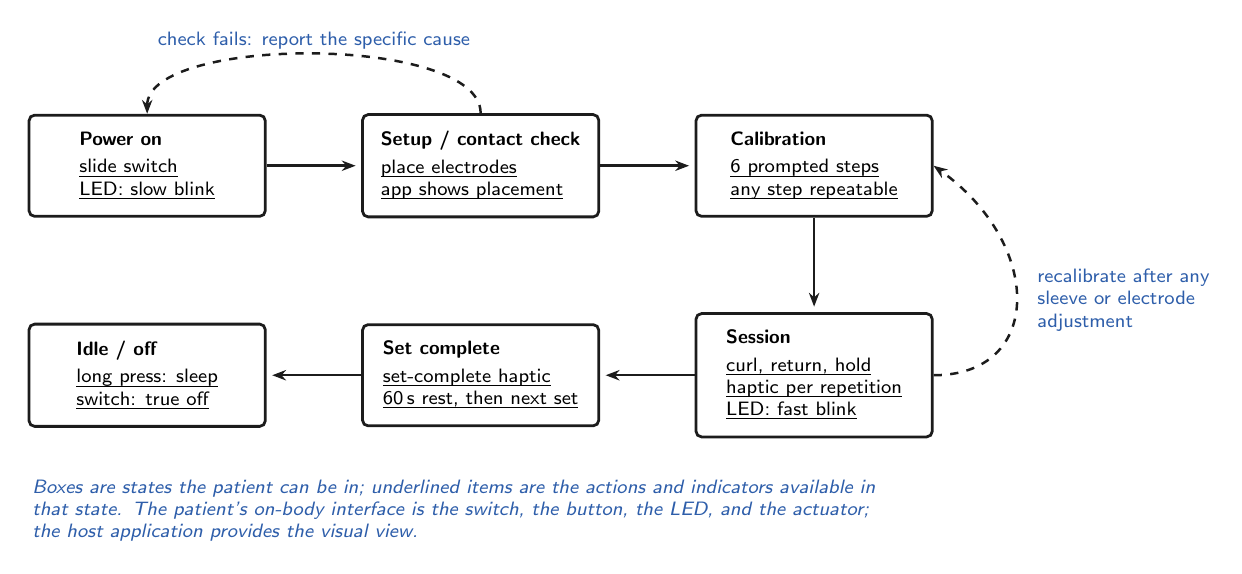
\begin{tikzpicture}[node distance=7mm]

\node[place] (p1) {\textbf{Power on}\\[2pt]
  \afford{slide switch}\\ \afford{LED: slow blink}};
\node[place, right=12mm of p1] (p2) {\textbf{Setup / contact check}\\[2pt]
  \afford{place electrodes}\\ \afford{app shows placement}};
\node[place, right=12mm of p2] (p3) {\textbf{Calibration}\\[2pt]
  \afford{6 prompted steps}\\ \afford{any step repeatable}};
\node[place, below=12mm of p3] (p4) {\textbf{Session}\\[2pt]
  \afford{curl, return, hold}\\ \afford{haptic per repetition}\\ \afford{LED: fast blink}};
\node[place, left=12mm of p4] (p5) {\textbf{Set complete}\\[2pt]
  \afford{set-complete haptic}\\ \afford{60\,s rest, then next set}};
\node[place, left=12mm of p5] (p6) {\textbf{Idle / off}\\[2pt]
  \afford{long press: sleep}\\ \afford{switch: true off}};

\draw[flow,shorten >=2pt] (p1.east) -- (p2.west);
\draw[flow,shorten >=2pt] (p2.east) -- (p3.west);
\draw[flow,shorten >=2pt] (p3.south) -- (p4.north);
\draw[flow,shorten >=2pt] (p4.west) -- (p5.east);
\draw[flow,shorten >=2pt] (p5.west) -- (p6.east);
\draw[flow, dashed] (p2.north) .. controls +(0,10mm) and +(0,10mm) .. (p1.north)
  node[midway,above,note]{check fails: report the specific cause};
\draw[flow, dashed] (p4.east) .. controls +(14mm,0) and +(14mm,-10mm) .. (p3.east)
  node[midway,right,note,xshift=2mm]{recalibrate after any\\sleeve or electrode\\adjustment};

\node[note, anchor=north west, text width=0.9\linewidth] at ($(p6.south west)+(0,-6mm)$)
  {\textit{Boxes are states the patient can be in; underlined items are the actions and
  indicators available in that state. The patient's on-body interface is the
  switch, the button, the LED, and the actuator; the host application provides
  the visual view.}};
\end{tikzpicture}
\caption{End-to-end session. A default prescription is three sets of twenty
repetitions with sixty seconds of rest between sets.}
\end{figure}

\subsection{Calibration}

Calibration runs as a sequence of short, separately commanded steps, so a failed
step can be repeated on its own without restarting the protocol. Total capture
time is approximately sixteen seconds on the single-channel prototype, or about
twenty-five including prompts --- against a Must of under thirty in \S3.2. The
triceps step returns with the second channel and adds nine.

\begin{table}[H]
\centering\small
\begin{tabularx}{\linewidth}{@{}p{24mm} p{11mm} p{40mm} X@{}}
\toprule
\textbf{Step} & \textbf{Time} & \textbf{Patient action} & \textbf{Captured, and pass condition} \\
\midrule
0. Setup & --- &
Sits; sleeve on; electrodes placed using the app's placement images &
Contact check: no channel saturated, mains pickup within limits, both IMUs
responding. Failure reports the specific cause (``press the electrode firmly'')
with the fault cue. \\[3pt]
1. Rest & 5\,s &
Arm relaxed at the side, completely still &
EMG resting mean and standard deviation, which set the muscle-on threshold, and
gyroscope bias for both IMUs. Rejected and repeated if movement is detected ---
movement here corrupts the bias, and therefore the joint angle, for the whole
session with no obvious symptom. \\[3pt]
2. Straight arm & 2\,s &
Straightens the arm \emph{as far as is comfortable} and holds still &
The $0^{\circ}$ reference pose, and the neutral-pose quaternions for both IMUs.
Rejected if not still during capture. \\[3pt]
3. Biceps maximum & $3\times3$\,s &
Elbow at $\sim$90$^{\circ}$, pushes up against a table and contracts the biceps &
Biceps 100\% reference, best of three attempts, each taken as the strongest
500\,ms window. Must be clearly above rest; if not, front-end gain is raised and
the step repeated. \\[3pt]
\textit{4. Triceps maximum} & \textit{$3\times3$\,s} &
\textit{Same posture, pushes down} &
\textit{Triceps 100\% reference, by the same method. Required by the
co-contraction score; Phase 2, with the second channel.} \\[3pt]
5. Range sweep & $\sim$6\,s &
Two slow, full-range curls &
Flexion axis, taken as the principal axis of the relative rotation over the
sweep, so sleeve alignment is not assumed; achievable $\theta_{\min}$ and
$\theta_{\max}$; baseline median frequency. \\
\bottomrule
\end{tabularx}
\end{table}

\paragraph{Findings incorporated from the 21 October session.}
\begin{itemize}
\item \tested Step 2 must instruct ``comfortable straight,'' not ``locked
straight.'' Calibrating against a hyperextended pose caused returns to finish
$10$--$12^{\circ}$ short of the finish threshold, so repetitions did not
complete.
\item \tested Step 4 was added because the co-contraction score normalises the
triceps channel as well and therefore requires its own reference. With one
channel there is no triceps to normalise, so the step is deferred rather than
dropped --- the reasoning survives, and returns with the hardware.
\item \tested A stillness check gates acceptance of steps 1 and 2. The rest step
also establishes gyroscope bias, and movement during it corrupts the joint angle
for the remainder of the session.
\item \tested Recalibration is required after any electrode or sleeve
adjustment. In the session log, resting EMG read approximately 40\% of the
calibrated maximum after the hardware shifted, which invalidates both the
activation scale and the ``relaxed between repetitions'' check.
\end{itemize}

\paragraph{Maximum contraction on an impaired limb.} Maximal effort is
inconsistent on a paretic limb, and a single poor attempt mis-scales every
subsequent measurement. Three mitigations apply: the measurement is the best of
up to three attempts rather than a single trial; if the best attempt fails to
exceed the rest baseline by a defined margin the device flags the reference as
unreliable and scales against the patient's own stored history instead; and a
clinician-supplied normalisation value, pushed from the host, supersedes the
measured one.

\paragraph{Persistence.} Results are written to NVS under a patient profile key
and survive power cycles. Steps 1, 2, and 5 are re-run every session, since they
reset gyroscope bias and IMU drift and absorb day-to-day variation in sleeve
placement. Steps 3 and 4 may be reused from the stored profile until it expires
or the patient requests recalibration.

\subsection{Repetition detection}

A repetition begins when the biceps activates and the arm rises past the start
threshold, and is counted when the arm has returned below the finish threshold
and been held still there for a configurable interval. Counting on the return
means the score covers the whole movement, including the eccentric phase, and
the confirming hold removes the ambiguity of counting on a threshold crossing
alone.

\begin{figure}[H]
\centering
\resizebox{\linewidth}{!}{%
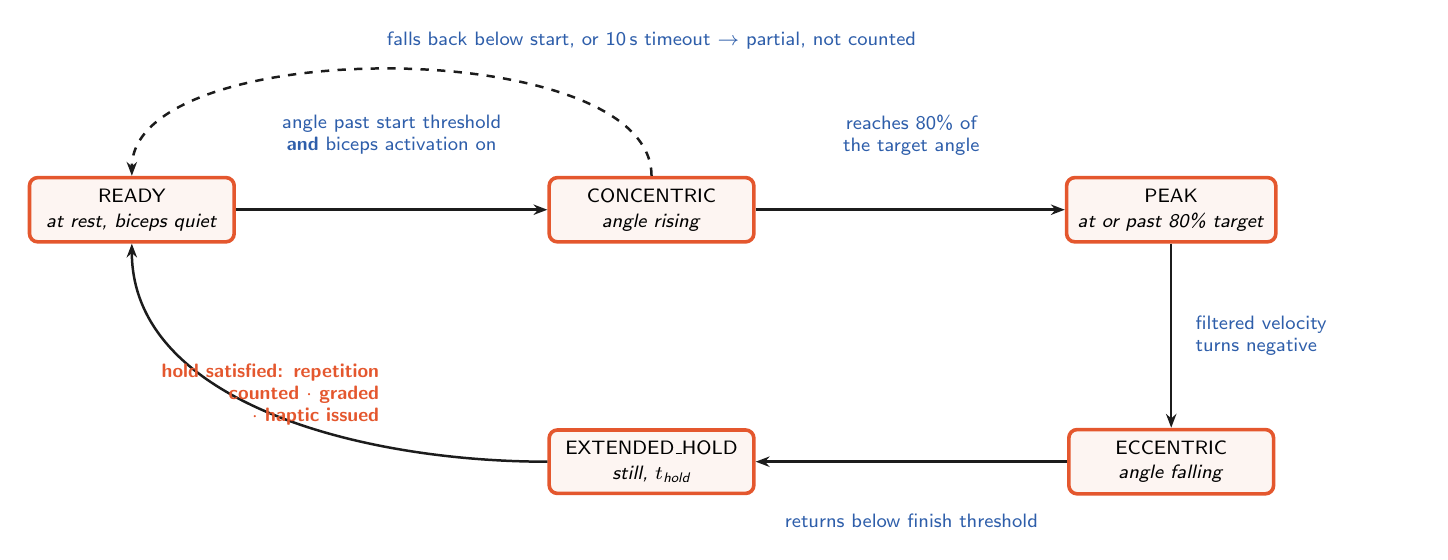
\begin{tikzpicture}[x=1cm,y=1cm]
\node[st,minimum width=26mm] (w)  at (0,0)       {READY\\[1pt]\textit{at rest, biceps quiet}};
\node[st,minimum width=26mm] (c)  at (6.6,0)     {CONCENTRIC\\[1pt]\textit{angle rising}};
\node[st,minimum width=26mm] (pk) at (13.2,0)    {PEAK\\[1pt]\textit{at or past 80\% target}};
\node[st,minimum width=26mm] (ec) at (13.2,-3.2) {ECCENTRIC\\[1pt]\textit{angle falling}};
\node[st,minimum width=26mm] (xh) at (6.6,-3.2)  {EXTENDED\_HOLD\\[1pt]\textit{still, $t_{\text{hold}}$}};

\draw[flow] (w.east) -- (c.west);
\node[note,align=center,text width=36mm] at (3.3,0.95) {angle past start threshold\\\textbf{and} biceps activation on};

\draw[flow] (c.east) -- (pk.west);
\node[note,align=center,text width=32mm] at (9.9,0.95) {reaches 80\% of\\the target angle};

\draw[flow] (pk.south) -- (ec.north);
\node[note,align=left,anchor=west,text width=28mm] at (13.45,-1.6) {filtered velocity\\turns negative};

\draw[flow] (ec.west) -- (xh.east);
\node[note,align=center,text width=34mm] at (9.9,-3.95) {returns below finish threshold};

\draw[flow] (xh.west) .. controls +(-2.4,0) and +(0,-2.0) .. (w.south);
\node[note,align=right,anchor=east,text width=32mm,color=marker] at (3.2,-2.35)
  {\textbf{hold satisfied: repetition\\counted $\cdot$ graded $\cdot$ haptic issued}};

\draw[flow,dashed] (c.north) .. controls +(0,1.8) and +(0,1.8) .. (w.north);
\node[note,align=center] at (6.6,2.15) {falls back below start, or 10\,s timeout $\rightarrow$ partial, not counted};
\end{tikzpicture}}
\caption{Repetition cycle. Start is gated on biceps activation; the repetition is
counted after the arm returns to the extended position and holds still there.}
\end{figure}

\begin{table}[!t]
\centering\small
\begin{tabularx}{\linewidth}{@{}p{34mm} p{32mm} X@{}}
\toprule
\textbf{Parameter} & \textbf{Default} & \textbf{Basis} \\
\midrule
Target angle & Therapist-set, $110^{\circ}$ &
\tested Volunteer repetitions peaked at $89$--$98^{\circ}$. Adequate for testing;
the therapist starts patients lower. \\
``Target reached'' & 80\% of target angle & Defines the peak criterion. \\
Start threshold & $15^{\circ}$ &
Configurable; $20^{\circ}$ for patients who cannot fully extend. \\
Finish threshold & $10^{\circ}$ ($5^{\circ}$ hysteresis) &
Configurable; $15^{\circ}$ alongside a raised start threshold. \\
\texttt{hold\_duration\_ms} & 1000\,ms, range 300--3000 &
The confirming hold at the extended position. Host-tunable, because an impaired
limb may not hold steadily for a full second. \\
\texttt{hold\_velocity\_thresh} & $15^{\circ}/\text{s}$ &
A hold requires the limb to be stationary, not merely below the threshold. \\
Biceps activation on & Envelope above rest mean $+\,3\sigma$ for 50\,ms; off below rest mean $+\,2\sigma$ for 100\,ms &
\tested Replaces a fixed 10\% threshold, and adapts to each session's own noise
floor. \\
Direction reversal & Filtered velocity $<0$, 5\,Hz low-pass &
\tested A fixed $-10^{\circ}/\text{s}$ was used to avoid jitter. \\
Tempo window & Therapist-set, 1.5--3.5\,s, start to finish &
\tested Volunteer repetitions ran 3.5--9\,s. The confirming hold is excluded
from the tempo measurement. \\
Repetition timeout & 10\,s without completion $\rightarrow$ partial &
\tested The session contained 16.6\,s and 24.7\,s ``repetitions.'' \\
Session structure & 3 sets $\times$ 20 repetitions, 60\,s rest &
Repetition goal is therapist-set and host-configurable. \\
\bottomrule
\end{tabularx}
\end{table}

\noindent
Thresholds are derived from the calibrated range of motion and the therapist's
target angle rather than from fixed anatomical angles. Counting remains
traceable: every count corresponds to a full excursion with the agonist active,
confirmed by a hold of defined duration. Sixteen scenarios pass in
\texttt{test/test\_rep.c} without hardware attached, among them a passively
swung arm that counts nothing, a long hold at the top that counts nothing, set
completion at the target, tempo scoring, and a shoulder hike that does not also
register as trunk lean.

\subsection{Grading and start-position checks}

Each repetition receives a score from 0 to 100, reported to the host after every
repetition. The patient receives only a pass/fail distinction, through the choice
of haptic pattern; the numerical score is shown in the application.

\begin{table}[H]
\centering\small
\begin{tabularx}{\linewidth}{@{}p{28mm} p{16mm} X@{}}
\toprule
\textbf{Component} & \textbf{Weight} & \textbf{Measure, and status} \\
\midrule
Range of motion & 1/3 & Peak angle divided by the therapist's target angle; also reported against the healthy reference corridor. \tested Working. \\
Tempo & 1/3 & Repetition duration, start threshold to finish threshold, against the prescribed window. \tested Working. \\
Smoothness & 1/3 & Count of velocity peaks exceeding 10\% of the repetition's peak velocity; a single peak scores 100. \tested Working. \\
\textit{Co-contraction} & \textit{0} & \textit{Overlap of biceps and triceps activation, evaluated only while the biceps is active. Needs the second channel and the triceps reference from calibration step 4; weighted zero until both exist.} \\
\midrule
\multicolumn{3}{@{}l}{\textbf{Deductions, applied after the mean; result clamped to 0--100}}\\
Shoulder compensation & $-20$ & \tested Upper-arm IMU rotates more than $\sim$20$^{\circ}$ from its calibration pose during the repetition. \\
Trunk lean & $-15$ & Common-mode rotation of both IMUs greater than $10^{\circ}$. \\
Momentum / arm swing & $-15$ & Upper-arm angular velocity above $30^{\circ}/\text{s}$ sustained for 200\,ms during the concentric phase. \\
\bottomrule
\end{tabularx}
\end{table}

\noindent
Components carry equal weight by default, and the score normalises by the
weights actually in force --- so a component weighted zero redistributes its
share across the rest rather than capping the best achievable score below 100.
Without that, a perfect repetition on the single-channel prototype would score
75, and the number on the therapist's screen would mean something different
from the number in this document.

\medskip
\noindent
Weights and deductions are host-configurable (\S5.9.1) so they can be tuned
against volunteer data without rebuilding firmware. Steadiness during the
confirming hold is computed and reported but does not contribute to the default
score; it is available as an optional fifth component.

\begin{table}[H]
\centering\small
\caption*{\textbf{Start-position and movement-quality checks}}
\begin{tabularx}{\linewidth}{@{}p{34mm} p{48mm} X@{}}
\toprule
\textbf{Condition} & \textbf{Detection} & \textbf{Response} \\
\midrule
Arm not returned near straight & Angle remains above the finish threshold & The hold never starts, so no repetition completes \\
Not relaxed between repetitions & Biceps envelope still above the activation threshold while at rest & Form cue; ``relax your arm'' shown in the app. \tested The 40\% resting EMG observed after a sleeve shift would trigger this. \\
Shoulder compensation & Upper-arm IMU rotated more than $\sim$20$^{\circ}$ from the calibration pose during the repetition & Repetition flagged; form cue \\
Passive swing & Angle rises with the biceps inactive & Repetition never starts \\
Sudden jolt & Acceleration spike on either IMU & That segment excluded from scoring \\
\bottomrule
\end{tabularx}
\end{table}

\noindent
Three behavioural rules apply regardless of the weights. Every completed
repetition is counted and then graded --- no repetition is discarded silently,
because a counter that fails to advance gives the patient no interpretable
information. A repetition flagged for compensation still counts toward the
repetition target: movement quality is expressed in the score, not in the
counter. And compensation detected at any point during the movement is latched
for that repetition and reported at the confirming hold, so feedback arrives at
a single predictable moment rather than interrupting the movement.

\medskip
\noindent
Two defects identified by the test suite are recorded here because both would
have manifested as implausible scores rather than as obvious failures. The
smoothness term initially rewarded slower movement, since mean change in
velocity scales with speed; it is now normalised by the movement's own mean
speed. The steadiness term initially penalised a deeper curl, because the
measurement window included the end of the ascent; the window now opens only
once the limb has settled.

\subsection{Haptic feedback}

Feedback is delivered by a single eccentric rotating mass (ERM) actuator ---
the Adafruit 1201 --- at the end of the confirming hold, when the patient is
stationary. An ERM's vibration frequency is coupled to its amplitude, so
``stronger'' also means ``faster'' and cannot carry independent meaning.
Patterns are therefore distinguished by \emph{rhythm} --- pulse count, width,
and gap --- and the six result cues are played at a single consistent
amplitude, which is also easier for a patient to learn than a set of intensity
gradations.

\medskip
\noindent
The DRV2605L's overdrive and active braking, applied from the stored
calibration, sharpen the onset and shorten the decay enough to make the pulses
and 70--80\,ms gaps below perceptible as distinct events rather than one
smeared buzz. Without a driver IC the gap floor would be roughly 120\,ms and
the vocabulary would have to be coarser.

\begin{table}[H]
\centering\small
\begin{tabularx}{\linewidth}{@{}p{38mm} p{42mm} X@{}}
\toprule
\textbf{Event} & \textbf{Pattern} & \textbf{Interpretation} \\
\midrule
Repetition counted, no fault &
One sharp click, 100\,ms &
The repetition counted and met the form, range, and tempo criteria. \\[3pt]
Repetition counted, form flagged &
Three pulses, 80\,ms on, 80\,ms off &
Counted, but incomplete range, outside the tempo window, or compensation
detected. \\[3pt]
Final repetition of the set &
Two 70\,ms pulses with 70\,ms gaps, then one 500\,ms pulse &
The repetition target has been reached. \\[3pt]
Rest now &
One 1000\,ms ramp up and down &
Fatigue flag raised. \\[3pt]
Fault &
Two 300\,ms pulses, 300\,ms apart &
Contact lost, sensor fault, or low battery. \\[3pt]
Button press acknowledged &
One 40\,ms tick &
Confirms every button press. \\[3pt]
80\% of the target angle &
One 30\,ms click at reduced level &
You may begin the return. The only cue delivered mid-movement. \\
\bottomrule
\end{tabularx}
\end{table}

\noindent
\tested The 21 October notes identified a collision between a double-pulse
``incomplete'' cue and a double-pulse fault cue. Using three pulses for a flagged
repetition resolves it and leaves the double pattern available for faults.

\medskip
\noindent
Each repetition receives exactly one of the first two patterns. On the
repetition that completes the set, the set-complete pattern follows the
per-repetition pattern after a 300\,ms gap, so the patient receives both the
quality result and confirmation that the set is finished.

\paragraph{Scheduling rules.} One cue plays at a time. A fault preempts a
playing cue and clears anything pending. A button-press tick is dropped if any
cue is playing, as is the soft click --- a waypoint the patient misses costs
nothing, whereas a result they miss costs the repetition. Otherwise a new cue
takes the single pending slot only if its priority exceeds that of the cue
already waiting. Priorities, lowest to highest: tick and soft click, repetition
result, set complete and rest, fault.

\paragraph{Timing.} The haptic task runs at the highest application priority on
a 1\,ms scheduler tick, and each pattern segment is timed from a hardware timer
so that pulse widths and gaps do not drift. The scheduler begins output on the
same call that receives a request, so it contributes no latency of its own.
Worst-case latency from the end of the confirming hold to perceptible vibration
is approximately 43\,ms, within the 50\,ms budget.

\paragraph{Cue blanking.} A cue's vibration couples into both the IMUs and the
electrodes. The proposal is for firmware to suspend IMU and EMG analysis for the
duration of each cue, so that a cue cannot be scored as a jolt or disturb the
following repetition. \textit{This needs agreement between the firmware and
algorithms owners before implementation (\S11.2).}

\paragraph{Host pattern test.} The host can fire any named pattern --- tick,
clean, flagged, set complete, rest, fault --- on demand, for bench verification
and for the through-fabric discrimination test with volunteers.

\paragraph{The soft click, and why it is shaped differently.} Settled on
22 October: a soft click fires at 80\% of the target angle to indicate that the
patient may begin the return. It is the only cue delivered while the patient is
moving, and everything about it is chosen so that it cannot be mistaken for a
result --- it is the shortest in the set, it plays at a reduced level, and it
skips the overdrive kick that gives the other cues their snap. The six result
cues keep their single consistent amplitude; the soft click sits deliberately
outside that class rather than breaking the rule within it.

\subsection{Hardware}

\begin{table}[H]
\centering\small
\begin{tabularx}{\linewidth}{@{}p{26mm} p{40mm} X@{}}
\toprule
\textbf{Function} & \textbf{Phase 1 (29 Oct)} & \textbf{Phase 2 (custom PCB)} \\
\midrule
MCU & ESP32-S3-DevKitC-1 v1.1 (N8R8) & ESP32-S3 module on the PCB \\
sEMG & MyoWare 2.0 $\times$ 1, RAW output, 3 electrodes & Integrated two-channel analogue front end with driven reference, 5 electrodes \\
ADC & ESP32-S3 internal ADC1, continuous DMA, $\sim$9.5 effective bits & TI ADS131M02 over SPI, 24-bit, simultaneous sampling \\
Motion & 2 $\times$ SparkFun BMI270 breakouts, SPI & 2 $\times$ BMI270 on board, SPI \\
Haptics & Adafruit DRV2605L breakout + Adafruit 1201 ERM & DRV2605L + ERM on board \\
Power & USB from the development board & LiPo cell, charge circuit, fuel gauge, slide switch on the battery line \\
Indication & On-board WS2812 & RGB status LED \\
User input & On-board BOOT button (GPIO0) & Dedicated button in the pod \\
\bottomrule
\end{tabularx}
\end{table}

\noindent
Firmware is written against an abstract acquisition interface with both the
internal-ADC and ADS131M02 backends in place, so moving from Phase 1 to Phase 2
is a single assignment at initialisation and touches nothing above the driver.

\paragraph{User button.} Short press: start or pause the session. Long press
(3\,s): sleep. Double press: recalibrate. Every press is confirmed by a haptic
tick.

\paragraph{Status indication.} The PCB carries an RGB LED, so device states are
colour-coded as well as blink-coded. A separate charge indicator is driven
directly from the charger's status pin and requires no firmware.

\begin{table}[H]
\centering\small
\begin{tabularx}{\linewidth}{@{}p{34mm} p{30mm} X@{}}
\toprule
\textbf{State} & \textbf{Colour} & \textbf{Pattern} \\
\midrule
Idle, advertising & Blue & Slow blink \\
Connected & Blue & Solid \\
Calibrating & Amber & Pulsing \\
Session running & Green & Fast blink \\
Battery below 15\% & Amber & Double blink every 2\,s \\
Fault & Red & Solid \\
\bottomrule
\end{tabularx}
\end{table}

\noindent
Below 15\% charge the device completes the current set, then stops and saves
rather than terminating mid-set.

\paragraph{Development pin assignment.} The map below applies to the Phase 1
build. On the custom PCB, EMG acquisition moves to the ADS131M02 on SPI2 with
its own chip select, and GPIO4, GPIO5 become available.

\begin{table}[H]
\centering\small
\begin{tabularx}{\linewidth}{@{}p{38mm} p{16mm} p{20mm} X@{}}
\toprule
\textbf{Signal} & \textbf{Pin} & \textbf{Peripheral} & \textbf{Note} \\
\midrule
EMG (biceps) RAW & GPIO4 & ADC1\_CH3 & 12\,dB attenuation, $\sim$0--3.1\,V window \\
\textit{EMG B (triceps) RAW} & \textit{GPIO5} & \textit{ADC1\_CH4} & \textit{Reserved; unused on the single-channel prototype} \\
Battery sense & GPIO7 & ADC1\_CH6 & 2:1 divider, read while continuous mode is paused \\
SPI SCK / MOSI / MISO & GPIO12 / 11 / 13 & SPI2 (FSPI) & 10\,MHz, shared by both IMUs \\
CS, upper-arm / forearm IMU & GPIO10 / 14 & GPIO out & \\
I\textsuperscript{2}C SDA / SCL & GPIO8 / 9 & I2C0 & DRV2605L only, 400\,kHz \\
Haptic PWM & GPIO6 & LEDC & DRV2605L IN/TRIG \\
Haptic enable & GPIO15 & GPIO out & Hard mute, bus-independent \\
Status LED & GPIO38 & RMT & On-board WS2812 \\
User button & GPIO0 & GPIO in & On-board BOOT button \\
\bottomrule
\end{tabularx}
\end{table}

\noindent
Pins avoided: GPIO19--20 (USB D$-$/D$+$), GPIO26--32 (SPI flash), and
GPIO33--37 (octal PSRAM on the N8R8 module).

\subsubsection*{5.7.1\quad Haptic driver: I\textsuperscript{2}C configuration, PWM drive}

\paragraph{Power-up sequence.} Reset the DRV2605L; leave standby; select ERM
drive mode (\texttt{N\_ERM\_LRA} $=0$ in Feedback Control, \texttt{0x1A}); set
the rated voltage and overdrive clamp from the actuator datasheet; run
auto-calibration; store the results in NVS; switch the mode register to PWM
input; then read back every configured register. A mismatch
fails the self-test before the session begins. If auto-calibration fails, the
driver falls back to the stored calibration; if none exists, initialisation
fails rather than running with unknown drive parameters. PWM cannot replace this
sequence --- it follows it.

\paragraph{PWM drive.} LEDC at 20\,kHz, 10-bit, with 50\% duty as zero drive and
deviation from 50\% setting amplitude. The output is held at zero drive before
the chip is switched into PWM mode, so the actuator cannot twitch during
configuration. The driver's overdrive and braking continue to shape each pulse
from the stored calibration while the PWM duty sets amplitude; this
configuration is to be confirmed against the datasheet during bring-up.

\paragraph{Enable pin.} Disabling holds EN low after first commanding zero
drive. Re-enabling re-sends the full configuration unconditionally, because the
chip loses its registers while EN is low.

\paragraph{Actuator limits.} Rated voltage and overdrive clamp are set from the
Adafruit 1201 datasheet before the first auto-calibration, starting
conservatively. The 1201 is a 2--5\,V part; 3.0\,V rated with a 3.3\,V clamp is
the current assumption in firmware, to be confirmed at bring-up. Wrong values
here produce a weak or buzzy actuator.

\begin{table}[H]
\centering\small
\caption*{\textbf{Why PWM, and what it costs}}
\begin{tabularx}{\linewidth}{@{}p{62mm} X@{}}
\toprule
\textbf{Gained} & \textbf{Given up} \\
\midrule
No bus transaction while the patient is moving, which is when connector and
cable flex on a worn sleeve make the I\textsuperscript{2}C link least reliable. &
The built-in effects library, which is selected by number over
I\textsuperscript{2}C. Every pattern must instead be shaped by hand. For the six
short patterns specified here this is a small amount of code and gives exact
control of pulse widths and gaps. \\[3pt]
Exact pulse timing. The specified patterns use 70--100\,ms pulses with 80\,ms
gaps, which the library's fixed envelopes do not reproduce precisely. &
One GPIO and one trace. \\[3pt]
Driver behaviour is retained: overdrive and active braking still operate from
the stored calibration in PWM input mode. &
A 20\,kHz switching signal routed near a microvolt-level analogue front end.
Mitigated because drive is active only during a cue of a few hundred
milliseconds, and cues fire when the patient is stationary at the confirming
hold. \\
\bottomrule
\end{tabularx}
\end{table}

\noindent
The practical conclusion is that PWM costs little and removes bus traffic from
the part of the session where the link is most exposed. A boot-time
I\textsuperscript{2}C failure remains possible, but it occurs while the patient
is stationary, it is detectable by the register read-back, and the step can be
retried; a failure mid-movement cannot be handled so cleanly. The effects
library remains available as a fallback should PWM shaping prove troublesome in
bring-up. The driver's EN pin is held by a GPIO, providing a hard mute
independent of the bus; if EN is used to sleep the driver between cues, the
configuration sequence is re-sent unconditionally on wake.

\subsection{Signal chain}

\begin{figure}[H]
\centering
\resizebox{\linewidth}{!}{%
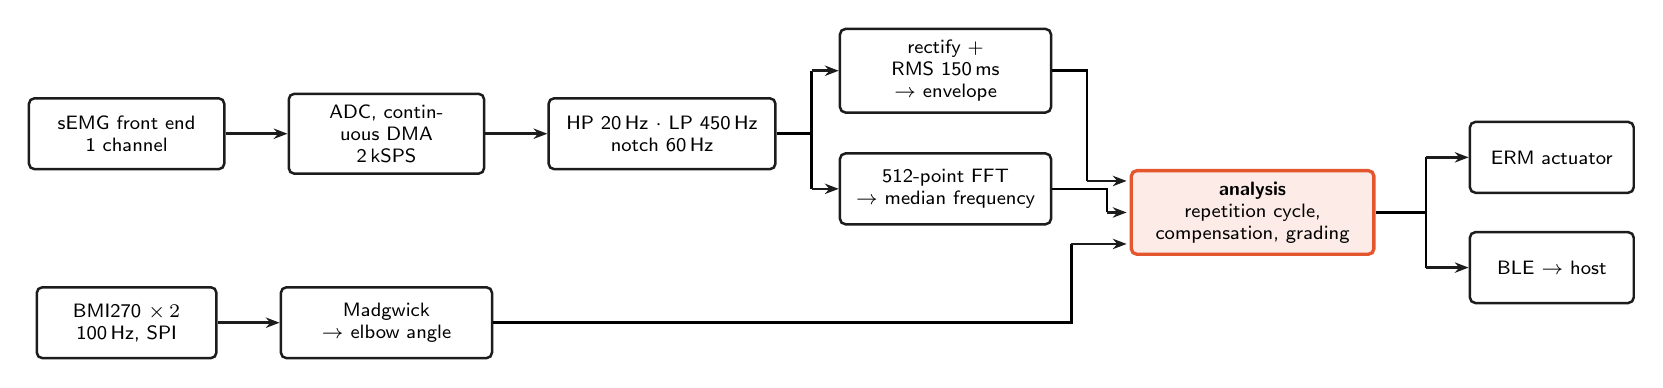
\begin{tikzpicture}[x=1cm,y=1cm]
% EMG lane
\node[blk,text width=22mm] (e) at (0,2.6)    {sEMG front end\\1 channel};
\node[blk,text width=22mm] (a) at (3.3,2.6)  {ADC, continuous DMA\\2\,kSPS};
\node[blk,text width=26mm] (d) at (6.8,2.6)  {HP 20\,Hz $\cdot$ LP 450\,Hz\\notch 60\,Hz};
\node[blk,text width=24mm] (r) at (10.4,3.4) {rectify + RMS 150\,ms\\$\rightarrow$ envelope};
\node[blk,text width=24mm] (m) at (10.4,1.9) {512-point FFT\\$\rightarrow$ median frequency};
% IMU lane
\node[blk,text width=20mm] (i) at (0,0.2)    {BMI270 $\times\,2$\\100\,Hz, SPI};
\node[blk,text width=24mm] (q) at (3.3,0.2)  {Madgwick\\$\rightarrow$ elbow angle};
% hub and outputs
\node[blk,text width=28mm,fill=marker!12,draw=marker,line width=1.2pt] (an) at (14.3,1.6)
  {\textbf{analysis}\\repetition cycle,\\compensation, grading};
\node[blk,text width=18mm] (h) at (18.1,2.3) {ERM actuator};
\node[blk,text width=18mm] (b) at (18.1,0.9) {BLE $\rightarrow$ host};

% EMG chain
\draw[flow] (e)--(a);
\draw[flow] (a)--(d);
\draw[line width=0.9pt] (d.east) -- (8.7,2.6);
\draw[line width=0.9pt] (8.7,3.4) -- (8.7,1.9);
\draw[flow] (8.7,3.4) -- (r.west);
\draw[flow] (8.7,1.9) -- (m.west);
% IMU chain
\draw[flow] (i)--(q);
% into the hub, three separate approaches, no shared segments
\draw[line width=0.9pt] (r.east) -- (12.2,3.4) -- (12.2,2.0);
\draw[flow] (12.2,2.0) -- (12.7,2.0);
\draw[line width=0.9pt] (m.east) -- (12.45,1.9) -- (12.45,1.6);
\draw[flow] (12.45,1.6) -- (12.7,1.6);
\draw[line width=0.9pt] (q.east) -- (12.0,0.2) -- (12.0,1.2);
\draw[flow] (12.0,1.2) -- (12.7,1.2);
% out of the hub
\draw[line width=0.9pt] (an.east) -- (16.5,1.6) -- (16.5,2.3);
\draw[flow] (16.5,2.3) -- (h.west);
\draw[line width=0.9pt] (16.5,1.6) -- (16.5,0.9);
\draw[flow] (16.5,0.9) -- (b.west);
\end{tikzpicture}}
\caption{Signal path. The haptic branch is independent of the BLE branch, so
feedback continues when the host connection is lost.}
\end{figure}

\noindent
Two choices in this chain are load-bearing. The front end delivers raw
band-limited sEMG rather than a rectified envelope, because envelope-only output
discards the frequency content that median-frequency fatigue tracking requires.
And acquisition runs in continuous DMA mode rather than one-shot conversions from
a timer callback, because the jitter introduced by the latter degrades the
spectral estimate that fatigue detection depends on.

\medskip
\noindent
\textbf{Fatigue detection.} Median frequency is computed from a 512-sample
Hann-windowed FFT with 50\% overlap, only while the activation envelope exceeds
threshold, and tracked as a linear regression across the set. Three consecutive
repetitions with a slope below the calibrated threshold raise a fatigue warning
and trigger the rest cue, once per set. Settled on 22 October: the warning
\textbf{advises and does not end the set}. The cue fires, the event is
reported, and what to do about it is the patient's and the therapist's
decision --- a device that ended a set on its own reading of a frequency trend
would be overruling the person doing the exercise.

\subsection{Host software}

The device is authoritative for every event it reports --- repetition counted,
compensation, fatigue, fault --- and the host displays those events rather than
re-deriving them from the raw stream.

\paragraph{Phase 1 host: Python.} A \texttt{bleak}-based client on a laptop
serves four functions: issuing control commands, plotting the live feature
stream, logging every received frame to CSV, and publishing repetition records
to the same MQTT topics the phone application will use, so the backend is
exercised before the phone application exists. The log is the input to offline
tuning of filter coefficients, thresholds, and grading weights, which is
required work regardless of host platform.

\smallskip
\noindent
Conditions attached to this substitution: the client uses the exact BLE layout
agreed for the phone application, so the phone client can replace it with no
firmware change; the 29 October demonstration is scoped to the live view rather
than the patient-facing game, which Python cannot exercise; and phone work
continues in parallel against the same specification.

\smallskip
\noindent
Implementation notes: the notification callback must do nothing but push into an
\texttt{asyncio.Queue}, with parsing and plotting in a separate task, or the BLE
connection stalls behind the plot; frames are capped at 180 bytes rather than the
244 a 247-byte MTU permits, because macOS caps ATT MTU at 185 and \texttt{bleak}
does not expose a portable MTU request; at approximately 10.4\,kB/s the raw
stream is well within the limits of every backend. Passkey pairing behaves
differently on macOS, so the passkey is disabled in prototype firmware builds.

\paragraph{Phase 2 host: Flutter application.} A single Flutter codebase
compiles to native Android and iOS builds, so both platforms are reachable from
one body of Dart code with a cross-platform BLE package. Android is the
development target, since deploying to an iOS device additionally requires macOS
tooling and a paid Apple developer account; iOS is added from the same codebase
once the Android build is stable. What the Python client cannot test ---
patient-facing user experience, the game, and platform BLE behaviour such as
connection interval, background operation, and permissions --- remains
phone-side work.

\paragraph{Pairing and connection loss.} The device advertises when idle, pairs
once using a six-digit passkey printed on the pod, and reconnects automatically
thereafter. Losing the link does not change the device state: acquisition,
repetition detection, grading, and all haptic feedback continue, and only the
transmit task idles. Repetition events are buffered to flash so they survive a
power loss; the full-rate raw stream is buffered in PSRAM. The host recovers the
missed range by sequence number on reconnection, and the device reports
explicitly if any data was genuinely lost.

\subsubsection*{5.9.1\quad Parameters settable from the host}

All parameters below are runtime-configurable over BLE, may be changed during a
session, take effect from the next repetition, and are stored in NVS and read
back for confirmation.

\begin{table}[H]
\centering\small
\begin{tabularx}{\linewidth}{@{}p{40mm} p{30mm} X@{}}
\toprule
\textbf{Parameter} & \textbf{Default} & \textbf{Purpose} \\
\midrule
\texttt{hold\_duration\_ms} & 1000\,ms (300--3000) & Duration of the confirming hold at the extended position. The primary tuning control during volunteer testing. \\
\texttt{rep\_target} & 20 (1--50) & Repetitions per set; determines when the set-complete pattern is issued. \\
\texttt{set\_count}, \texttt{rest\_seconds} & 3, 60\,s & Session structure. \\
\texttt{target\_angle} & $110^{\circ}$ & Therapist-set; the peak criterion is 80\% of this value. \\
\texttt{start\_angle}, \texttt{finish\_angle} & $15^{\circ}$, $10^{\circ}$ & Raised together for patients who cannot fully extend. \\
\texttt{tempo\_min}, \texttt{tempo\_max} & 1.5\,s, 3.5\,s & Prescribed tempo window. \\
Compensation thresholds & $20^{\circ}$, $10^{\circ}$, $30^{\circ}/\text{s}$ & Shoulder, trunk, and momentum sensitivity. \\
Grading weights and deductions & Equal weights, \S5.5 & Tuned against volunteer data. \\
\texttt{raw\_stream\_enable} & On during tuning & Switches the full-rate raw stream without affecting results or events. \\
Haptic pattern test & --- & Fires a named pattern on demand for bench verification. \\
\bottomrule
\end{tabularx}
\end{table}

%==============================================================================
\section{Performance metrics and acceptance criteria}

\begin{table}[H]
\centering\small
\begin{tabularx}{\linewidth}{@{}p{32mm} X@{}}
\toprule
\textbf{Metric} & \textbf{Acceptance test} \\
\midrule
Joint angle accuracy & Within $5$--$10^{\circ}$ of a goniometer at $0^{\circ}$, $45^{\circ}$, $90^{\circ}$, $135^{\circ}$ \\
Calibration robustness & Each step repeatable individually; movement during steps 1--2 rejected; a hyperextended step 2 does not prevent repetitions from completing; the whole protocol completes in under 30\,s \\
Repetition counting & Ten deliberate repetitions counted as exactly ten, on three consecutive runs; a passively swung arm produces no count. \tested Both pass in \texttt{test/test\_rep.c} \\
Partial rejection & A repetition abandoned mid-range, and one exceeding the 10\,s timeout, both reported as partial and not counted \\
Feedback latency & Haptic delivered within 50\,ms of the confirming hold completing \\
Pattern discrimination & A blindfolded team member identifies all seven patterns correctly 10/10 times, through fabric, and never mistakes the soft click for a result \\
Pattern timing accuracy & Pulse widths and gaps within 10\% of specification, measured on the PWM line (proposed tolerance) \\
Driver configuration integrity & Zero register read-back mismatches across 50 consecutive power cycles (proposed) \\
No cue overlap & No two patterns drive the actuator at once; covered by host-side tests and a bench capture \\
Link independence & Cues continue with the BLE link disconnected mid-set \\
Cue interference & No measurable increase in the EMG noise floor or IMU artefacts attributable to a cue (proposed) \\
Compensation detection & Staged shoulder elevation flagged, the repetition still counted, and the score reduced \\
Contact-fault detection & A deliberately lifted electrode raises the fault cue with its specific cause \\
Fatigue detection & Median-frequency trend falls measurably across a deliberately fatiguing set, the rest cue fires once, and the set continues \\
Set completion & Set-complete pattern fires on the repetition reaching \texttt{rep\_target}, for targets of 5 and 20 \\
Parameter configuration & \texttt{hold\_duration\_ms} and \texttt{rep\_target} changed from the host take effect on the next repetition and survive a power cycle \\
Raw stream control & Raw stream disabled and re-enabled mid-session without interrupting results or events \\
Link robustness & 60\,s logged with zero sequence gaps; a forced disconnection loses no data after recovery \\
Signal quality & Clipping counter reads zero at maximum effort once front-end gain is set \\
Battery life & Two hours of continuous operation; below 15\% the device completes the set, then stops and saves \\
\bottomrule
\end{tabularx}
\end{table}

%==============================================================================
\section{Milestones}

Aligned to the course schedule. Weekly lab notebook entries are published to the
project website by noon each Friday, and the team meets the instructor and TAs
during the Thursday lab.

\begin{table}[H]
\centering\small
\begin{tabularx}{\linewidth}{@{}p{22mm} p{40mm} X@{}}
\toprule
\textbf{Date} & \textbf{Course deliverable} & \textbf{Project milestone} \\
\midrule
Oct 22 & PRD on website, noon & This document; design forks closed \\
Oct 23--28 & --- & EMG channel live; DSP chain verified; both IMUs on SPI; elbow angle against a goniometer; all seven haptic patterns verified on a scope and through fabric; BLE stream logged \\
Oct 29 & Rapid prototype on website, noon & Phase 1 demonstration: full signal path on the development board with MyoWare \\
Oct 30--Nov 2 & --- & PCB schematic complete and reviewed \\
Nov 3 & Status presentation & 10-minute update: goals, architecture, state, remaining risks \\
Nov 4--7 & --- & PCB ordered; volunteer data collection for the reference corridor begins \\
Nov 10 & Peer review 1, noon & --- \\
Nov 11--21 & --- & Grading tuned against volunteer data; sleeve and pod mechanical design; battery and charging \\
Nov 24--Dec 1 & --- & PCB bring-up; integration onto the sleeve \\
Dec 2--8 & --- & Full-system integration; two complete demo rehearsals \\
Dec 10 & Final demo and presentation & Live demonstration per \S3.1 \\
Dec 15 & Final report, peer review 2, noon & ACM double-column technical report \\
\bottomrule
\end{tabularx}
\end{table}

%==============================================================================
\section{Team responsibilities}

\begin{table}[H]
\centering\small
\begin{tabularx}{\linewidth}{@{}p{34mm} X@{}}
\toprule
\textbf{Member} & \textbf{Primary areas} \\
\midrule
Qian (Andy) Cai & Hardware: schematic capture, PCB layout, component selection, board bring-up, power and charging. Owns the development boards. \\
Aidan Goodman & Firmware architecture: acquisition layer, DSP chain, BLE service and the host interface contract, test suites. \\
Rusha Maiti & Algorithms and validation: calibration protocol, repetition detection and grading parameters, prototype testing and volunteer data collection. \\
Eyerusalem Earl & Host software and integration: Python client, Flutter application, backend topics, mechanical integration of sleeve and pod. \\
\midrule
Rotating duties & Schedule management, weekly lab notebook, purchasing and reimbursement forms, website upkeep. \\
\bottomrule
\end{tabularx}
\end{table}

\noindent
Assignments are primary areas rather than exclusive ownership; integration work
is shared. \textit{To be confirmed by the team at the 22 October lab and
corrected here if different.}

%==============================================================================
\section{Materials, budget, and outside help}

\begin{table}[H]
\centering\small
\begin{tabularx}{\linewidth}{@{}X r r@{}}
\toprule
\textbf{Item} & \textbf{Status} & \textbf{Cost (\$)} \\
\midrule
ESP32-S3 development boards ($\times$3) & Owned & 0 \\
SparkFun BMI270 IMU breakouts ($\times$2) & Ordered & 37.00 \\
Adafruit DRV2605L haptic drivers ($\times$2) & Ordered & 15.90 \\
\rowcolor{good!8} Adafruit 1201 ERM actuators ($\times$5) --- the selected actuator & Ordered & 9.75 \\
MyoWare 2.0 sensor, cable shield, electrodes, electrode cable & Ordered & 65.15 \\
\midrule
\textit{Subtotal, Phase 1} & & \textit{127.80} \\
\midrule
\textit{Second MyoWare channel --- no longer needed; the custom PCB carries both} & \textit{Not ordered} & \textit{0} \\
Custom PCB fabrication and assembly & To order & 150--250 \\
PCB components (front end, ADS131M02, BMI270, DRV2605L, regulators, passives) & To order & $\sim$80 \\
LiPo cell, charge circuit, fuel gauge & To order & $\sim$25 \\
Ag/AgCl electrodes, consumable stock & To order & $\sim$30 \\
Compression sleeve, fabric, fasteners, 3D-printed pod & To order & $\sim$40 \\
\midrule
\textbf{Projected total} & & \textbf{$\sim$510--610} \\
\bottomrule
\end{tabularx}
\end{table}

\noindent
Figures beyond the Phase 1 subtotal are estimates and will be revised as
quotations arrive. Purchases are reimbursed through the course form.

\medskip
\noindent
Two decisions of 22 October reduce the outstanding spend: the ERM units already
purchased are the production actuator, so no LRA order is needed, and the
single-channel prototype removes the second MyoWare module. Both were in the
Phase 1 ``to order'' column in v1.4.

\paragraph{Facilities and tools.} Lab bench in CSE 003E; oscilloscope and bench
supply; Altium Designer for PCB design; a 3D printer for the pod and electrode
housings; a goniometer for angle validation.

\paragraph{Outside help needed.}
\begin{itemize}
\item A physical or occupational therapist, for review of the exercise protocol,
realistic target angles and tempo ranges for patients, and what a clinician
would want to see reported.
\item Healthy volunteers for the reference corridor and for staged compensation
testing.
\item PCB fabrication and assembly service, per the course instructions.
\end{itemize}

%==============================================================================
\section{Risks and mitigations}

\subsection{Project risks}

\begin{table}[H]
\centering\small
\begin{tabularx}{\linewidth}{@{}p{40mm} p{14mm} X@{}}
\toprule
\textbf{Risk} & \textbf{Impact} & \textbf{Mitigation} \\
\midrule
PCB fabrication or assembly delay & High & Order by the first week of November; the Phase 1 development-board build remains a complete working fallback for the final demonstration \\
Custom analogue front end underperforms the MyoWare reference & High & Bring up the PCB front end against the MyoWare signal as a reference; keep the MyoWare path wirable \\
Triceps channel arrives only with the PCB & Medium & Co-contraction is unscored until then, and the donning check cannot detect a reversed sleeve. Both paths are written and guarded on one constant, so the PCB enables them rather than requiring new work \\
Electrode contact instability on a moving sleeve & High & Continuous contact monitoring with a fault cue; short leads; compression and foam backing; recalibration prompt \\
Component availability & Medium & Order early; select parts with second sources where possible \\
Volunteer availability for data collection & Medium & Recruit within the course cohort; begin collection in early November \\
Scope creep from the phone application and game & Medium & Phase 1 scoped to the live view; phone work proceeds in parallel and is not on the critical path \\
Actuator rated voltage or overdrive clamp set wrongly & High & Set from the Adafruit 1201 datasheet before the first auto-calibration; start conservatively \\
Driver configuration fails or is lost (boot-time I\textsuperscript{2}C error, or an EN sleep resetting the chip) & High & Register read-back self-test; configuration re-sent unconditionally on wake; stored-calibration fallback \\
Patterns indistinguishable through fabric & High & Distinguish by rhythm and length rather than intensity; test through fabric early; tune with volunteers \\
ERM spin-up smears the shortest pulses (the 40\,ms tick and the 30\,ms soft click) & Medium & Overdrive kick and active braking from the stored calibration; verify on a scope; lengthen the cue if needed \\
Haptic timing stretched by radio activity & Medium & The haptic task shares core 0 with the BLE host. Measure pulse widths on the PWM line with BLE active; if marginal, move segment timing to a hardware timer \\
20\,kHz PWM couples into the EMG front end & Medium & Drive only during short cues at the stationary hold; route the trace away from the front end; compare the noise floor with and without cues \\
Cue vibration scored as an IMU jolt, or disturbing the next repetition & Medium & Cue blanking (\S5.6), pending team agreement \\
Fault-state mute silences the fault cue & Medium & Play the fault cue to completion before cutting EN (\S5.2) \\
Single points of knowledge in the team & Low & Weekly lab notebook; code and design files in the shared repository \\
\bottomrule
\end{tabularx}
\end{table}

\subsection{Implementation hazards}

\begin{description}[leftmargin=0pt,style=unboxed,itemsep=5pt]

\item[\textcolor{marker}{Electrode contact drift during a session.}] \tested The
single largest source of bad data in the 21 October session. A sleeve or
electrode shift after calibration raised resting EMG to roughly 40\% of the
calibrated maximum, invalidating the activation scale, the co-contraction score,
and the ``relaxed between repetitions'' check simultaneously.

\item[\textcolor{marker}{BMI270 configuration upload.}] The BMI270 ships inert
and requires an approximately 8\,kB configuration blob to be uploaded before it
produces data. A device that reports the correct chip ID but returns only zeros
typically indicates a configuration upload that failed silently. The
initialisation routine verifies \texttt{INTERNAL\_STATUS} $=$ \texttt{0x01} after
upload, and the self-test fails explicitly if it does not.

\item[\textcolor{marker}{BMI270 SPI mode entry.}] The device powers up in
I\textsuperscript{2}C mode regardless of board configuration. On the breakouts:
ADR jumper fully open (this selects SPI), I\textsuperscript{2}C pull-up jumpers
cut, and header pins mapped SCL$\rightarrow$SCK, SDA$\rightarrow$PICO,
ADR$\rightarrow$POCI, CS$\rightarrow$CS. The driver then performs a dummy read of
register \texttt{0x00} and allows CSB to rise, which latches SPI mode. Omitting
this produces invalid data on all subsequent transfers.

\item[\textcolor{marker}{Front-end gain and clipping.}] Clipping degrades the
median-frequency estimate while leaving the activation envelope apparently
plausible, so it is not detectable by inspection. The firmware maintains a
per-channel clipping counter, reported in telemetry, and gain is set against that
counter rather than visually. Calibration step 3 raises gain automatically when
the maximum contraction reads too low.

\item[\textcolor{marker}{Internal ADC noise in Phase 1.}] The ESP32-S3 internal
ADC provides roughly 9.5 effective bits, against approximately 110\,dB of dynamic
range for the ADS131M02. Adequate for validating the chain, not for the product.
If the signal appears unusable after filtering, investigate in this order:
front-end gain, then electrode contact and reference placement, then ADC
attenuation and calibration.

\item[\textcolor{marker}{Yaw drift without a magnetometer.}] Absolute heading is
unobservable with this sensor set, so elbow angle is always the relative
rotation between the two IMUs with respect to their neutral-pose references.
Mitigations: the per-session re-zero, and a rest-phase re-anchor to gravity
whenever both IMUs report low angular velocity and acceleration near $1\,g$ for
more than 300\,ms --- which the confirming hold now guarantees once per
repetition.

\item[\textcolor{marker}{Gyroscope bias corruption at calibration.}] \tested
Movement during the rest step corrupts gyroscope bias and therefore the joint
angle for the whole session, with no obvious symptom. The stillness gate exists
to prevent this.

\item[\textcolor{marker}{PSRAM configuration.}]
\texttt{CONFIG\_SPIRAM\_MODE\_OCT} must be set; the default quad mode causes an
N8R8 module to report no PSRAM. The session buffer is allocated with
\texttt{heap\_caps\_malloc(size, MALLOC\_CAP\_SPIRAM)} and verified at boot.

\item[\textcolor{marker}{Buffer sizing.}] At 2\,kSPS across two channels plus IMU
data the raw stream is approximately 648\,kB per minute, while only 300--350\,kB
of internal SRAM remains free once the BLE stack is loaded. Buffering is tiered:
DMA landing buffers, an 8-second live ring in SRAM, and the full session in
PSRAM. Repetition events are additionally written to flash so they survive power
loss.

\item[\textcolor{marker}{Mains interference.}] Battery operation limits 60\,Hz
pickup, but lead length makes the notch filter necessary, and the setup contact
check measures pickup explicitly. A 180\,Hz harmonic notch sits behind a
compile-time flag.

\item[\textcolor{marker}{Trunk lean is inferred.}] Detected as common-mode
rotation of the two arm IMUs rather than measured. A trunk-mounted IMU would be
required to measure it, and is not in scope.
\end{description}

%==============================================================================
\section{Out of scope for this quarter}

\begin{plainbox}
\begin{itemize}
\item \textbf{The patient-facing game.} Development may proceed in parallel, but
it is not demonstrated and the Python client cannot exercise it.
\item \textbf{The therapist dashboard.} The device-side data path and the MQTT
topics are in place and exercised from the Python client; the dashboard itself
is later work.
\item \textbf{Remote adjustment of exercise targets from a clinician portal.}
Parameters are adjustable from the local host only.
\item \textbf{Wi-Fi connectivity and an on-device web interface.} BLE is the
single host transport.
\item \textbf{Machine-learning models.} Repetition detection uses deterministic
thresholds, and no labelled dataset yet exists --- the current thresholds are
what will generate the labelled boundaries a model would require. Learned
quality scoring is the natural second version.
\item \textbf{Dry and textile electrode evaluation.} Snap Ag/AgCl only.
\item \textbf{Multiple patient profiles per device.}
\item \textbf{Wrist-substitution detection.} Not observable with this sensor set;
it requires a third IMU on the hand.
\item \textbf{Clinical validation and any diagnostic claim.} See \S13.
\end{itemize}
\end{plainbox}

%==============================================================================
\clearpage
\section{Decisions and open questions}

\subsection{Decisions settled on 22 October}

\noindent
The four below were taken after the firmware had been brought into line with
v1.4, and each reverses or closes something that document left open.

\begin{table}[H]
\centering\small
\begin{tabularx}{\linewidth}{@{}p{30mm} X@{}}
\toprule
\textbf{Question} & \textbf{Decision} \\
\midrule
Prototype channel count & \textbf{One} EMG channel, on the biceps. Three electrodes. The triceps channel and the co-contraction score arrive with the custom PCB, which carries both without a second module or a second reference. \\[3pt]
Actuator & \textbf{ERM} for the full production cycle. The v1.4 move to an LRA is reversed: the ERM units are already purchased, the DRV2605L's overdrive and braking make the specified rhythms workable, and nothing in the pattern vocabulary depends on resonance tracking. \\[3pt]
Soft click at 80\% of target & \textbf{Yes.} Added as a seventh pattern, deliberately shaped so it cannot be mistaken for a result (\S5.6). \\[3pt]
Fatigue warning & \textbf{Advises only.} The cue fires and the event is reported; the set continues. A device that ended a set on its own reading of a frequency trend would be overruling the person doing the exercise. \\
\bottomrule
\end{tabularx}
\end{table}

\subsection{Decisions carried forward from v1.4}

\begin{table}[H]
\centering\small
\begin{tabularx}{\linewidth}{@{}p{30mm} X@{}}
\toprule
\textbf{Question} & \textbf{Decision} \\
\midrule
Haptic drive path & I\textsuperscript{2}C configuration at power-up, switching to PWM drive immediately and for the remainder of the session. Rationale and costs in \S5.7.1. \\
Where a repetition is counted & On return to the extended position, after a configurable confirming hold. Tempo therefore covers the full excursion, and the hold provides the stationary moment that feedback and gravity re-anchoring both need. \\
Tempo versus hold steadiness & Tempo is scored; hold steadiness is computed and reported but is not part of the default score. \\
Status indicator & RGB LED on the custom PCB, giving colour-coded states as well as blink patterns. \\
Phone platform & Flutter, which compiles to both Android and iOS from one codebase. Android first, iOS added from the same source. \\
Phase 1 sensing & MyoWare 2.0 for the 29 October prototype; the custom front end follows on the PCB. \\
Haptic timing & Patterns shaped by hand over PWM rather than selected from the driver's effects ROM, for exact control of pulse widths and gaps. \\
Raw data stream & Sent at full rate but switchable, so tuning sessions record it and ordinary use does not. \\
Data lost to a dropout & Replayed by sequence number on reconnection. \\
Flagged repetitions & Count toward the repetition target; quality is expressed in the score. \\
Live parameter changes & All listed parameters may be changed mid-session, taking effect from the next repetition. \\
\bottomrule
\end{tabularx}
\end{table}

\subsection{Still open}

\begin{table}[H]
\centering\small
\begin{tabularx}{\linewidth}{@{}p{13mm} p{62mm} X@{}}
\toprule
\textbf{By} & \textbf{Question} & \textbf{Blocks} \\
\midrule
Oct 23 & Adafruit 1201 rated voltage and overdrive clamp from the datasheet & Driver auto-calibration values. Firmware assumes 3.0\,V rated, 3.3\,V clamp until confirmed \\
Oct 24 & Agree cue blanking: suspend IMU and EMG analysis for the duration of each cue? & Scoring behaviour around cues; firmware and algorithms owners both affected. The soft click makes this slightly more pressing, since it is the one cue that fires while the patient is moving \\
Oct 25 & Electrode sites confirmed on the biceps belly & Volunteer data collection; not a firmware-structure dependency \\
Oct 25 & Shared-reference front end verified on the bench against separate references & Five-electrode layout; PCB schematic \\
Oct 25 & Haptic pattern timing measured on the PWM line with BLE active & Whether segment timing can stay on the scheduler or must move to a hardware timer \\
Nov & Demonstration covers elbow flexion only, or adds wrist flexion and extension? & Electrode siting; sleeve design \\
Nov & Battery capacity, fuel gauge part, and charge circuit against the two-hour target & Pod design \\
\bottomrule
\end{tabularx}
\end{table}

\subsection{The BLE interface, in plain terms}

Over BLE the device advertises a set of named channels, and the host subscribes
to the ones it needs. Each channel has an identifier and a defined message
layout. The identifiers themselves are arbitrary --- any value works, provided
firmware and host use the same one --- so they are not a design decision; they
are generated once and recorded in a shared header file. The decisions that
matter are what the device sends, how often, and what the host may change.

\begin{table}[H]
\centering\small
\begin{tabularx}{\linewidth}{@{}p{34mm} X@{}}
\toprule
\textbf{Channel} & \textbf{Content and rate} \\
\midrule
Commands (host $\rightarrow$ device) & Start, stop, run a named calibration step, set parameters, read parameters, test a haptic pattern, enable or disable the raw stream, set clock, power off \\
Live features (device $\rightarrow$ host) & Envelope, joint angle, state, repetition count and whether the agonist is active, at 20\,Hz on air; analysis runs internally at 50\,Hz \\
Results (device $\rightarrow$ host) & Per-repetition score and flags, plus events: partial repetition, compensation, fatigue, contact fault, set complete \\
Raw data (device $\rightarrow$ host) & Full-rate EMG and IMU samples, $\sim$10.4\,kB/s, switchable \\
Status (device $\rightarrow$ host) & State, battery, signal quality, and the range of data the device still holds \\
Recovery (device $\rightarrow$ host) & Replay of data missed during a disconnection, requested by range, served below the live stream in priority \\
Configuration (device $\rightarrow$ host) & The parameters of \S5.9.1 as the device holds them, read back so the host can confirm a change took effect \\
\bottomrule
\end{tabularx}
\end{table}

\noindent
All multi-byte values are little-endian, and every sample carries a timestamp
from a single monotonic device clock. The host sends its own wall-clock time on
connection; the device records the offset and reports it, but never adjusts its
own clock, since altering the sampling clock would corrupt the spectral analysis.

%==============================================================================
\section{Changes from the October project proposal}

\begin{table}[H]
\centering\small
\begin{tabularx}{\linewidth}{@{}p{36mm} p{36mm} X@{}}
\toprule
\textbf{Proposal} & \textbf{Current} & \textbf{Reason} \\
\midrule
MyoWare 2.0 and ADC~15 Click as the final front end & One MyoWare for Phase 1; integrated two-channel front end with ADS131M02 on the PCB & Single integrated board. Three electrodes for the prototype; five on the PCB, which adds the triceps pair and shares one driven reference \\
Single maximum-contraction step & Separate biceps and triceps maxima, the triceps deferred to Phase 2 & \tested The co-contraction score normalises the triceps and needs its own reference; with one channel there is nothing to normalise yet \\
90\,s calibration & Six steps, $\sim$19\,s of capture, individually repeatable & A failed step should not require restarting the protocol \\
Haptic within 200\,ms of the compensating movement & Feedback within 50\,ms of the confirming hold completing & Feedback is scheduled rather than reactive \\
Two IMUs on I\textsuperscript{2}C & Two IMUs on SPI & No sensor data on a shared bus \\
Phone to cloud to therapist dashboard & Python host publishing to the same MQTT topics; Flutter application in parallel; dashboard later & Logging is required for tuning regardless, and the backend is exercised early \\
Haptic patterns unspecified & Seven defined patterns, with distinct fault and set-complete cues, a mid-movement soft click, and explicit priority and preemption rules & \tested The original double-pulse scheme collided with the fault cue; patterns are distinguished by rhythm \\
ERM actuator & \textbf{ERM retained} & An LRA was proposed in v1.4 and reversed on 22 October: the units are purchased, and the DRV2605L's overdrive and braking already make the specified rhythms workable \\
Fixed repetition protocol & Hold duration, repetition target, thresholds, tempo window, and grading weights configurable from the host & Required for tuning against volunteer data without rebuilding firmware \\
\bottomrule
\end{tabularx}
\end{table}

%==============================================================================
\section{Safety, ethics, and standards}

RehabSense is a research prototype and makes no diagnostic claim. It is battery
powered and is not connected to mains-powered equipment while worn; the analogue
rail is cut in hardware whenever the device is charging. Testing is limited to
team members and consenting healthy volunteers; validation with stroke patients
is future work and outside the scope of this course. Session data is
health-related, and the current design keeps raw data on the device and on the
local host machine.

\paragraph{Applicable standards.} Were RehabSense developed as a product rather
than a course prototype, the governing standard would be
\textbf{IEC 60601-1} for the basic safety and essential performance of medical
electrical equipment, together with \textbf{IEC 60601-1-11} for equipment used in
the home healthcare environment. The relevant requirement for this design is
patient isolation: the electrodes are in direct skin contact, so leakage current
limits and the prohibition on a mains path to the patient apply directly, which
is why the device is battery powered and the analogue rail is disconnected
during charging. Classification under the FDA framework would likely place a
device of this kind as a Class II powered muscle stimulator-adjacent or
biofeedback device requiring 510(k) clearance; the project makes no such claim
and is not submitted for it.

%==============================================================================
\appendix
\section{Related research (EE 542)}

\paragraph{Cifrek et al., ``Surface EMG based muscle fatigue evaluation in
biomechanics'' (2009)~\cite{cifrek}.} This review surveys methods for detecting
localised muscular fatigue from surface EMG, with emphasis on spectral indices:
as a muscle fatigues, the power spectrum of its EMG shifts toward lower
frequencies, and the mean and median frequency of that spectrum fall measurably
over a sustained contraction. The paper also catalogues the practical
difficulties --- non-stationarity of the signal during dynamic contractions,
sensitivity to electrode placement, and the need for adequate bandwidth and
sampling. Its influence on this project is direct and structural. It is the
reason the system samples raw, band-limited EMG at 2\,kSPS per channel rather
than the pre-rectified envelope a sensor module can supply: the envelope
discards exactly the spectral content the fatigue index depends on. It is also
why median frequency is computed only while the activation envelope exceeds
threshold and is tracked as a regression across a set rather than evaluated on a
single window, and why clipping is counted and reported rather than assumed
absent.

\paragraph{Hermens et al., ``Development of recommendations for SEMG sensors and
sensor placement procedures'' (2000)~\cite{hermens}.} This paper reports the
SENIAM project's consensus recommendations for surface EMG sensor design and
placement, including bipolar electrode configurations, an inter-electrode
distance on the order of 20\,mm, placement over the muscle belly aligned with
the fibre direction, and reference placement on electrically inactive tissue.
Its influence on this project appears in the electrode layout: two electrodes
at approximately 20\,mm spacing along the belly of the biceps, with a reference
on the bony prominence at the elbow, and the triceps pair added on the same
pattern when the custom PCB arrives. It also motivates the donning check, since
the recommendations only hold if the sensors are actually where the protocol
assumes.

\medskip
\noindent
With two channels that check is a comparison --- the biceps channel must exceed
the triceps during a prompted curl, which catches a reversed sleeve and says so
specifically. With one channel there is nothing to compare against, so the
prototype instead requires the envelope to rise while the elbow flexes: enough
to catch a lifted, misplaced or dead electrode, not enough to name a reversed
sleeve, and the message the patient sees says so rather than claiming more. Finally, it is the basis for treating electrode siting as a
fixed, documented procedure illustrated in the application rather than something
left to the patient's judgement.

%==============================================================================
\begin{thebibliography}{9}\small
\bibitem{cdc} Centers for Disease Control and Prevention, \emph{Stroke Facts}.
  Accessed Oct.\ 12, 2026. \url{https://www.cdc.gov/stroke/facts.htm}
\bibitem{deluca} C.\ J.\ De Luca, \lq\lq Myoelectric manifestations of localized
  muscular fatigue in humans,\rq\rq\ \emph{Crit.\ Rev.\ Biomed.\ Eng.}, vol.\ 11,
  no.\ 4, pp.\ 251--279, 1984.
\bibitem{cifrek} M.\ Cifrek, V.\ Medved, S.\ Tonkovi\'c, and S.\ Ostoji\'c,
  \lq\lq Surface EMG based muscle fatigue evaluation in biomechanics,\rq\rq\
  \emph{Clin.\ Biomech.}, vol.\ 24, no.\ 4, pp.\ 327--340, 2009.
\bibitem{hermens} H.\ J.\ Hermens, B.\ Freriks, C.\ Disselhorst-Klug, and
  G.\ Rau, \lq\lq Development of recommendations for SEMG sensors and sensor
  placement procedures,\rq\rq\ \emph{J.\ Electromyogr.\ Kinesiol.}, vol.\ 10,
  no.\ 5, pp.\ 361--374, 2000.
  \url{https://doi.org/10.1016/S1050-6411(00)00027-4}
\bibitem{madgwick} S.\ O.\ H.\ Madgwick, A.\ J.\ L.\ Harrison, and
  R.\ Vaidyanathan, \lq\lq Estimation of IMU and MARG orientation using a
  gradient descent algorithm,\rq\rq\ in \emph{Proc.\ IEEE ICORR}, 2011, pp.\ 1--7.
\bibitem{bmi270} Bosch Sensortec, \emph{BMI270 datasheet}.
  \url{https://www.bosch-sensortec.com/media/boschsensortec/downloads/datasheets/bst-bmi270-ds000.pdf}
\bibitem{ads} Texas Instruments, \emph{ADS131M02: two-channel, simultaneously
  sampling, 24-bit delta-sigma ADC}, datasheet.
\bibitem{drv} Texas Instruments, \emph{DRV2605L haptic driver for ERM and LRA
  actuators with built-in library and smart loop architecture}, datasheet.
\end{thebibliography}

\end{document}
